\documentclass[10pt,journal]{IEEEtran}

\usepackage{graphicx}
\usepackage{cite}
\usepackage{amsmath}
\usepackage{tensor}

\DeclareMathOperator{\Tr}{Tr}
\DeclareMathOperator{\cov}{cov}

\begin{document}

\title{Smoothing and Interpolating Noisy GPS Data with Tension Splines}

\author{Jeffrey~J.~Early and Adam~Sykulski%
\thanks{Jeffrey J. Early is with NorthWest Research Associates, 4118 148th Ave NE, Redmond, WA 98052, USA (email: jearly@nwra.com) } %
\thanks{Adam Sykulski is with the Department of Statistical Science, University College London, Gower Street, London WC1E 6BT, UK (email: a.sykulski@ucl.ac.uk)}%
\thanks{Manuscript submitted February 29th, 2050.} }


\markboth{IEEE TRANSACTIONS ON SIGNAL PROCESSING}{}

\maketitle

\begin{abstract}
A technique is developed for smoothing and interpolating noisy GPS data using B-splines with tension. An interpolating B-spline basis set of arbitrary order is reformulate using knot placement, rather than the traditional approach of adding additional constraints on the coefficients. Adding tension to the interpolating spline to smooth noisy data is shown to be equivalent to a maximum likelihood problem on the velocity statistics of the underlying process. This insight allows for nearly optimal choice in smoothing parameter, and also shows the limitations of smoothing splines. Finally, we show how to modify the smoothing operator to account for the non-Gaussianity of GPS errors and reject outliers.


We show how the tension condition routinely employed in smoothing splines can be restated as a maximum likelihood problem and then how the tension parameter can be chosen based on physical reasoning. The GPS errors appear to be non-Gaussian, so we use a t-distribution in the maximum likelihood.
1. We reformulate the not-a-knot boundary condition in terms of spline placement, rather than additional conditions on the constrained problem.
2. We show how the tension condition routinely employed in smoothing splines can be restated as a maximum likelihood problem and then how the tension parameter can be nearly optimally chosen.
3. We show how to modify the smoothing operator to account for the non-Gaussianity of GPS errors and reject outliers.

\end{abstract}

\begin{IEEEkeywords}
IEEE, IEEEtran, journal, \LaTeX, paper, template.
\end{IEEEkeywords}



%%%%%%%%%%%%%%%%%%%%%%%%%%%%%%%%%%%%%%%%%%%%%%%%%%%%%%%%%%%%%%%%%%%%%
% MAIN BODY OF PAPER
%%%%%%%%%%%%%%%%%%%%%%%%%%%%%%%%%%%%%%%%%%%%%%%%%%%%%%%%%%%%%%%%%%%%%

%%%%%%%%%%%%%%%%%%%%%%
%
\section{Introduction}
%
%%%%%%%%%%%%%%%%%%%%%%

\begin{itemize}
    \item degrees-of-freedom vs u scaling from knot paper is useful for initial estimate.
    \item confirm that dof/2 knot placement doesn't hurt anything
    \item new information occurs at roughly dt*dof.
    \item order of spline should \emph{not} continue the slope, but should be steeper. The reason is because this generates incoherent part of solution, which simply serves to add noise.
\end{itemize}

Global positioning system receivers (now commonly referred to as `a GPS') are used in literally billions of devices around the the world to track positions. The quality of the position data can be quite good, with accuracies down to a few meters, but real world effects (such as atmospheric conditions and sky blockages) can significantly increase the errors \cite{faa2016-report}. Kalman filters are often employed to reduce these errors because they can be run in real time \cite{brown1997-book}, but it is often still the case that the data  contains outliers, noisy positions, and infrequent or inconsistent sampling that requires a combination of smoothing and interpolation.

Observations from GPS receivers return positions $x_i$ at times $t_i$ that differ from the true positions $x(t_i)$ by some noise $\epsilon_i \equiv x_i - x(t_i)$. The primary goal of \emph{smoothing} is to find the true position $x(t_i)$ not contaminated by the noise, while the primary goal of \emph{interpolating} is to find the true position $x(t)$ between observation times.

The impetus for this manuscript arose from the analysis of position data from nine free floating ocean surface buoys (drifters) equipped with GPS receivers recording locations every 30 minutes. For our analysis we require the position data be evenly spaced and synchronized in time across the drifters (interpolation). The dataset also clearly shows outliers (position jumps of hundreds of meters) that must be removed (smoothing). However, it is also important that the power spectrum is not significantly altered in the process of interpolating and smoothing.

Given the ubiquity of this basic problem, there are certainly many approaches to finding the true path $x(t)$---the approach taken here is to use maximum likelihood. The central idea of maximum likelihood is to ask ``Given a particular path $x(t)$, what is the probability that this dataset $(t_i,x_i)$ could have occurred?'' \cite{press1992-book}. The goal is then to find the path that is most likely to have produced that dataset.

Conceptually there are two major pieces needed to solve this problem,
\begin{enumerate}
\item we need to specify the form of the path---a model, and
\item we need to specify at least one probability distribution function (PDF) for some aspect of the signal or errors.
\end{enumerate}

The approach taken in this manuscript is to specify the model using smoothing splines. In section \ref{sec:interpolation} we review b-splines and introduce the canonical interpolating spline that is used as the underlying model for path $x(t)$ throughout this manuscript. Section \ref{sec:maximum_likelihood} formulates the maximum likelihood problem in terms of the error in positions and the velocity of the particle. This is shown to be equivalent to using a tensioned smoothing spline. Section \ref{sec:optimal_parameter} shows how the optimal tension parameter can be chosen directly from the data time series.

This manuscript is written with the broad goal of serving as a practical guide to smoothing noisy GPS data, to that end we introduce our primary dataset of interest in section \ref{sec:drifter_data_set}. We show that the GPS errors are not Gaussian distributed, but t-distributed and show how to modify the technique for a t-distribution. Finally, section \ref{sec:outliers} shows how outliers can be removed from the dataset before fitting with a tension spline.

%%%%%%%%%%%%%%%%%%%%%%
%
\section{Interpolation Spline}
\label{sec:interpolation}
%
%%%%%%%%%%%%%%%%%%%%%%

\begin{figure*}[t]
  \centerline{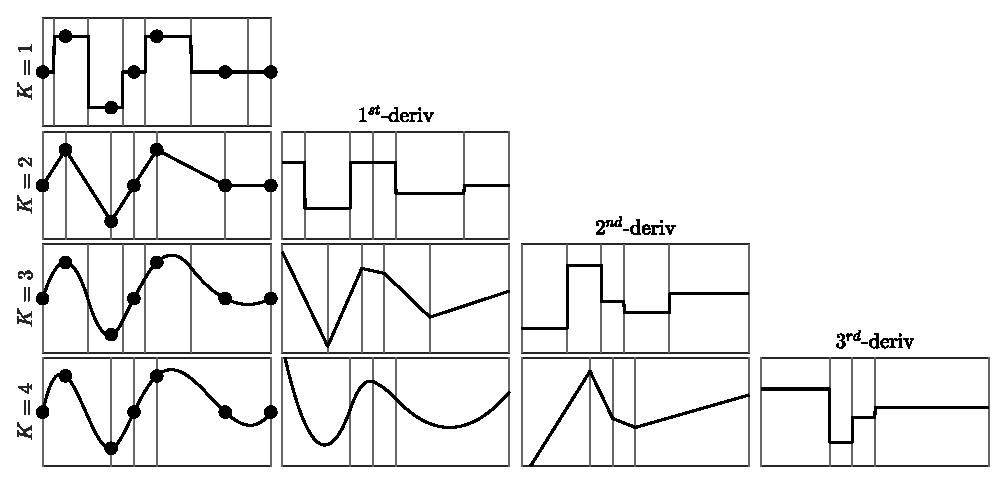
\includegraphics[width=39pc,angle=0]{figures/interpolation}}
  
  \caption{This shows an example of interpolating between 7 data points. The data points are shown as circles, and the interpolated function is shown as a solid black lines. We show four different orders of interpolation $K=1..4$ (rows) and their nonzero derivatives (columns). The thin vertical grey lines are the knot points.}
  \label{interpolation}
\end{figure*}

Assume that we are given $N$ observations of a particle position $(t_i,x_i)$ with no errors. The simplest possible form of interpolation would be a nearest neighbor method that assigns the position of the particle to the nearest observations in time. The resulting interpolated function $x(t)$ is a polynomial of \emph{order} $K=1$ (piecewise constant), shown in the top row of figure \ref{interpolation}. The next level of sophistication is to assume a constant velocity between any two observations and use that to interpolate positions between observations, second row of figure \ref{interpolation}. This also means that we now have a piecewise constant function $\frac{dx}{dt}$ that represents the velocity of the particle, shown in the second row, second column of figure  \ref{interpolation}. This is a polynomial function of order $K=2$.

It is slightly less obvious how to proceed to a polynomial of order $K=3$. With $N$ data points we can construct a piecewise constant acceleration (the second derivative) using the $N-2$ independent accelerations, but where to place $\emph{knot points}$ that define the boundaries of the regions and how to maintain continuity is slightly less clear. The approach taken here is to use B-splines.

%%%%%%%%%%%%%%%%%%%%%%
\subsection{B-Splines}
%%%%%%%%%%%%%%%%%%%%%%

A B-spline (or basis spline) of \emph{order} $K$ (\emph{degree} $S=K-1$) is a piecewise polynomial that maintains nonzero continuity across $S$ knot points. The knot points are a nondecreasing collection of points in time that we will denote with $\tau_i$. The basic theory is well documented in \cite{deboor1978-book}, but here we will present a reduced version specifically tailored to our needs.

The $m$-th B-spline of order $K=1$ is defined as,
\begin{equation}
X^1_m(t) \equiv \begin{cases}
1      & \text{if $ \tau_m \leq t < \tau_{m+1}$}, \\
0     & \text{otherwise}.
\end{cases}
\end{equation}
This is the rectangle function as shown in the first row, first column of figure \ref{bsplines}. If we are given $P$ knot points, then we can construct $P-1$ B-splines of order $K=1$, although notice that if a knot point is repeated this will result in a splines that is zero everywhere. To represent an interpolating function $x(t)$ for the $N$ observations of a particle position $(t_i,x_i)$ we define $N+1$ knot points as,
\begin{equation}
\tau_m = \begin{cases}
t_1      & \text{$m=1$}, \\
t_{m-1} + \frac{t_{m-1}-t_m}{2}	  & \text{$1<m \leq N$}\\
t_N     & \text{$m>N$}.
\end{cases}
\end{equation}
This will create $N$ independent basis functions that provide support for the region $t_i \leq t \leq t_N$ (provided the last spline is defined to include the last knot point). The interpolating function $x(t)$ is defined as $x(t) \equiv  X^1_m(t) \xi^m$ where the coefficients $\xi^m$ are found by solving $X^1_m(t^i) \xi^m = x^i$. The result of this process is shown in figure \ref{interpolation} for 7 irregularly spaced data points.

All higher order B-splines are defined by recursion,
\begin{equation}
X^K_m(t) \equiv \frac{t - t_m}{t_{m+K-1} - t_m} X^{K-1}_m(t) + \frac{t_{m+K}-t}{t_{m+K} - t_{m+1}} X^{K-1}_{m+1}(t).
\end{equation}
This recursion formula takes two neighboring lower order splines and ramps the left one up over its nonzero domain and ramps the right one down over its nonzero domain. The result of this process is to create splines that span across one additional knot point at each order, and maintain continuity across one more derivatives. Examples are shown in figure \ref{bsplines}.

Any knot points that are repeated $T$ times will result in an a total of $T-1$ splines of order one that are everywhere zero. This has the effect of introducing discontinuities in the derivatives for higher order splines. For our purposes, we will only use this feature to prevent higher order splines from crossing the boundaries. For $K=2$ order splines we will use $N+2$ knot points at locations,
\begin{equation}
\tau_m = \begin{cases}
t_1      	& \text{$m \leq 2$}, \\
t_{m-1}	& \text{$2 < m < N$}\\
t_N 		& \text{$m \geq N$}.
\end{cases}
\end{equation}
This creates a knot point at every observation point, but repeats the first and last knot point. This has the effect of terminating the first and last spline at the boundary and creating $N$ second order B-splines, $X^2_m(t)$. Once again the interpolating function $x(t)$ is defined as $x(t) \equiv  X^2_m(t) \xi^m$ where the coefficients $\xi^m$ are found by solving $X^2_m(t^i) \xi^m = x^i$. The second row of figure \ref{interpolation} shows an example.

This process can be continued to higher and higher order B-splines. For splines that are of \emph{even} order, we create $N+K$ knots points with
\begin{equation}
\tau_m^{\text{$K$-even}} = \begin{cases}
t_1      	& \text{$m \leq K$}, \\
t_{m-K/2}	& \text{$K < m < N$}\\
t_N 		& \text{$m \geq N$}
\end{cases}
\label{even-knots}
\end{equation}
and for splines that are \emph{odd} order, we create $N+K$ knot points with,
\begin{equation}
\tau_m^{\text{$K$-odd}} = \begin{cases}
t_1      	& \text{$m \leq K$}, \\
t_{m-\frac{K+1}{2}} + \frac{t_{m-\frac{K+1}{2}}-t_{m-\frac{K+1}{2}+1}}{2}	& \text{$K < m \leq N$}\\
t_N 		& \text{$m > N$}
\end{cases}
\label{odd-knots}
\end{equation}
The knot points are chosen specifically to create $N$ splines for the $N$ data points such that the interpolated function $x(t)$ crosses all $N$ observations $(t_i,x_i)$. The path $x(t)$ is the \emph{canonical interpolating spline of order K}. Examples are shown in figure \ref{interpolation}.

\begin{figure}
  \centerline{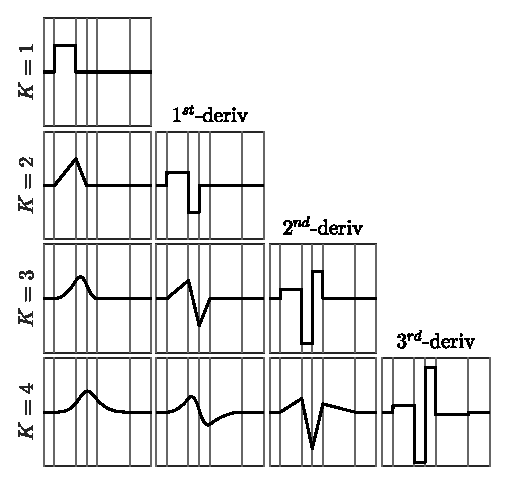
\includegraphics[width=19pc,angle=0]{figures/bsplines}}
  \caption{This shows an example B-spline and its derivatives (columns) for orders $K=1..4$ (rows).}
  \label{bsplines}
\end{figure}

The knot placements in \ref{even-knots} and \ref{odd-knots} are equivalent to the \textit{not-a-knot} boundary conditions described in \cite{deboor1978-book} and used in the cubic spline implementation in \texttt{Matlab}. In the usual formulation of the not-a-knot boundary condition, the knot positions do not change as a function of spline order, and therefore additional constraints have to be added at each order---specially, the requirement that the highest derivative maintain continuity near the boundaries. In the formulation here, these constraints are implicit in \ref{even-knots} and \ref{odd-knots}.


%%%%%%%%%%%%%%%%%%%%%%
%
\section{Smoothing Spline}
\label{sec:maximum_likelihood}
%
%%%%%%%%%%%%%%%%%%%%%%

A typical starting point for maximum likelihood is to establish the probability distribution function (PDF) of the errors, $\epsilon_i \equiv x_i - x(t_i)$. The canonical example in one-dimension is to assume that the error in our position measurements are Gaussian and are therefore drawn from the following probability distribution
\begin{equation}
\label{gaussian_pdf}
p_g(\epsilon|\sigma_g) = \frac{e^{-\frac{1}{2}\frac{\epsilon^2}{\sigma_g^2}} }{\sigma_g \sqrt{ 2 \pi}}
\end{equation}
where $\sigma_g$ is the standard deviation. This assumption alone places no assumptions on the signal itself, only on the structure of the noise.

The probability of the observed data given some model $x(t)$ is,
\begin{equation}
\label{max-gaussian}
P \sim \prod_{i=1}^{N}  \exp \left[ -\frac{1}{2} \left( \frac{x_i - x(t_i)}{\sigma_i} \right)^2 \right] \Delta x
\end{equation}
where we've allowed the standard deviation of the error, $\sigma_i$, to differ at each time $t_i$.

Maximizing the probability function in equation \ref{max-gaussian} is also the same as minimizing its argument (called the penalty function),
\begin{equation}
\label{least-squares}
\phi = \frac{1}{N}\sum_{i=1}^{N} \left( \frac{x_i - x(t_i)}{\sigma_i} \right)^2 .
\end{equation}
Stated in this way is plain to see that this is the same as asking for the `least-squares' fit of the errors.


%%%%%%%%%%%%%%%%%%%%%%
\subsection{Smoothing spline penalty function}
%%%%%%%%%%%%%%%%%%%%%%

The model used here will be the canonical interpolating spline of order $K$ described in section \ref{sec:interpolation}. Of course, we've chosen our knot points such that the model intersects each observations and this certainly maximizes equation \ref{max-gaussian} (and minimize equation \ref{least-squares}) because all the errors are zero, but the resulting distribution of errors (a delta function at zero) doesn't look anything like the assumed Gaussian distribution. Thus, if we want the error distribution that we get out to look like that which we assumed, it also necessary to \emph{constrain} the problem in some way.

The smoothing spline augments the penalty function of equation \ref{least-squares} by adding a global constraint on the $m$-th derivative of the resulting function,
\begin{equation}
\label{smoothing-spline}
\phi =  \frac{1}{N}\sum_{i=1}^{N} \left( \frac{x_i - x(t_i)}{\sigma_i} \right) ^2 + \lambda_m \int_{t_1}^{t_N} \left(\frac{d^m x}{dt^m}\right)^2 \, dt.
\end{equation}
If $\lambda_m \rightarrow 0$ then this reduces to the least-squares fit in equation \ref{least-squares}, but if $\lambda_m \rightarrow \infty$ then this forces the model to an $m$-th order polynomial (e.g., when $m=2$, the model will forced to be a straight line because it has no second derivative). The smoothing spline was first introduced in modern form by \cite{reinsch1967-nm}, but according to \cite{deboor1978-book} the idea dates back to \cite{whittaker1923-pems}.

The first term of equation \ref{smoothing-spline} is proportional to the sample variance,
\begin{equation}
\label{sample_variance}
\hat{\sigma}^2  \equiv \frac{1}{N} \sum_{i=1}^{N} \left( x_i - x(t_i) \right) ^2,
\end{equation}
which is expected to scale like
\begin{equation}
\label{sample_variance_variance}
\hat{\sigma}^2 = \frac{d-1}{d} \sigma^2
\end{equation}
where $d$ is the number of degrees of freedom (reference Adam? It's on the wikipedia page on Cochran's theorem). For a large number of degrees of freedom the sample variance matches the true variance, but as will be discussed in section \ref{sec:optimal_parameter} this distinction is key to optimal parameter choice.

There is a very simple physical interpretation for the second term in equation \ref{smoothing-spline}. Consider the case where $m=1$ so that the smoothing spline is a constraint on velocity. When averaged over the integration time, the integral produces the root mean square velocity, $u_{\textrm{rms}}$, which means that the second term scales like $u_{\textrm{rms}}^2 T$ where $T\equiv t_N-t_1$. In general, where $x^{(m)}_{\textrm{rms}}$ is the root-mean-square of the $m$-th derivative, this means that
\begin{equation}
\label{lambda}
\lambda_m = \frac{d-1}{d} \frac{1}{ \left(x^{(m)}_{\textrm{rms}}\right)^2 T}.
\end{equation}
The interpretation of the smoothing spline is therefore that the two terms are balanced by a relative weighting of the sample variance and mean-square of the $m$-th derivative of the physical process.

% Combining equations \ref{sample_variance} and \ref{sample_variance_variance} means that the first term in equation \ref{smoothing-spline} scales like $N \frac{d_{\textrm{var}}-1}{d_{\textrm{var}}}$.

% This estimate for the sample \emph{variance} can be compared with our estimate for the sample \emph{mean}, the error for which is expected to scale like $SE = \frac{\sigma}{\sqrt{d_{\textrm{mean}}}}$. When choosing the optimal parameter in section \ref{sec:optimal_parameter}, we will use the fact that the degree-of-freedom in the sample variance should be the same as the degrees-of-freedom in the standard error.

%%%%%%%%%%%%%%%%%%%%%%
\subsection{Smoothing spline maximum likelihood}
%%%%%%%%%%%%%%%%%%%%%%

The penalty function for the smoothing spline (\ref{smoothing-spline}) can be restated in terms of maximum likelihood. Assume that in addition to knowing about how the measurement errors are distributed like in equation \ref{max-gaussian}, that we also know how the velocity of underlying physical process is distributed. For example, in geophysical turbulence it has been shown that the velocity probability distribution function is like a two-sided exponential \cite{bracco2000-pf}. Here we will consider the case where the velocity PDF is Gaussian. Stated as maximum likelihood, this means that at \emph{any given instant} (not just the times of observation) we expected the model velocity to look Gaussian. We can discretize the problem by sampling the velocity $Q$ at times $t_q = t_1 + q \Delta t_q$ where $\Delta t_q=\frac{t_N-t_1}{Q-1}$ and $q=0..Q-1$. The maximum likelihood is thus stated as,
\begin{equation}
\label{gaussian-max-likelihood}
\begin{split}
P \sim \prod^N _{i=1}\exp \left[ -\frac{1}{2} \left( \frac{x_i - x(t_i)}{\sigma_i} \right)^2 \right] \\\cdot \prod^{Q}_{q=1} \exp \left[  - \frac{1}{2} \left(  \frac{u(t_q)}{\sigma_u} \right)^2 \right] \Delta x
\end{split}
\end{equation}
which is simply the joint probability of the error distribution from equation \ref{max-gaussian} and the velocity distribution of the underlying physical process. Writing this as a penalty function (after converting the product of exponentials into exponentials of sums), we have that
\begin{equation}
\label{smoothing-spline-pdf}
\phi =\frac{d}{d-1}  \frac{1}{N} \sum^N _{i=1}  \left( \frac{x_i - x(t_i)}{\sigma_i} \right)^2 + \frac{1}{\sigma_u^2 T} \sum^{Q}_{q=1}  u^2(t_q) \Delta t_q.
\end{equation}
where we've renormalized the error PDF and the velocity PDF to have equal weighting regardless of number of points. Apart from the discretization of the integral, equation \ref{smoothing-spline} is the same as the penalty function for a smoothing spline, equation \ref{smoothing-spline-pdf}.

The implication of this result is that adding tension to the penalty function is equivalent to assuming that one of the higher order derivatives in the model (e.g., velocity) is Gaussian. This is therefore making an assumption about the underlying \emph{physical process} of the model. This is in contrast to the first term which is entirely a statement about \emph{measurement noise}.

A second implication is that the tension spline can be easily modified to accommodate a mean value in tension, as shown in appendix \ref{mean_tension}. 

%%%%%%%%%%%%%%%%%%%%%%
%
\section{Optimal parameter estimation} \label{sec:optimal_parameter}
%
%%%%%%%%%%%%%%%%%%%%%%

For a given choice of $m$ and $\lambda_m$ the minimum solution to equation \ref{smoothing-spline} can be found analytically (see \cite{teanby2007-mg} and our appendix~\ref{sec:numerical_implementation}). Once the solution is found the smoothing matrix $\mathbf{S_\lambda}$ is defined as the matrix that takes the observations $\mathbf{x}$ and maps them to their smooth values, $\mathbf{\hat{x}} = \mathbf{S_\lambda} \mathbf{x}$.

The free parameter in this model, $\lambda_m$, is a relative weighting between the two terms in equation \ref{smoothing-spline} and choosing its optimal value can be done by minimizing the expected mean square error \cite{craven1979-nm},
\begin{align}
\label{MSE}
    \textrm{MSE}(\lambda) =& \frac{1}{N} || \left( \mathbf{S_\lambda} - I \right) \mathbf{x} ||^2 + \frac{2 \sigma^2}{N}  \Tr \mathbf{S_\lambda} - \sigma^2
\end{align}
where $||\cdot||^2$ is the Euclidean norm and $\Tr$ indicates the trace.

The mean square error in equation \ref{MSE} is a combination of the sample variance and the variance of the mean. The first terms in equation \ref{MSE} is mean sample variance from equations \ref{sample_variance} and \ref{sample_variance_variance} written in this notation it can be related to the degrees of freedom with,
\begin{equation}
    \left(1-\frac{1}{d} \right)\sigma^2 = \frac{1}{N} || \left( \mathbf{I} - \mathbf{S_\lambda} \right) \mathbf{x} ||^2.
\end{equation}
The second term is proportional to twice the variance of the mean. As shown in \cite{teanby2007-mg}, the quantity $\mathbf{S_\lambda} \Sigma$ is the covariance matrix with the squared standard error along the diagonal. Thus, the mean standard error is given by $\frac{1}{N} \Tr \left( \mathbf{S_\lambda} \Sigma \right)$ and can be related the degrees of freedom with,
\begin{equation}
    \frac{\sigma^2}{d} = \frac{1}{N} \Tr \left( \mathbf{S_\lambda} \Sigma \right).
\end{equation}


In the 50 years since \cite{reinsch1967-nm} was published, a number of different methods have been proposed for choosing the optimal value of $\lambda_m$ in equation \ref{smoothing-spline}. One approach is cross-validation \cite{wahba1978-jrss-b,craven1979-nm} which is essentially a form of bootstrapping, where the optimal parameter is determined by minimizing the error with data points not included in the fit. Another approach is to determine the number of degrees of freedom expected in the sample variance of equation \ref{sample_variance}. Both \cite{reinsch1967-nm} and \cite{teanby2007-mg} argue that the tension should be adjusted so that the sample variance is roughly the expected variance, $\hat{\sigma}^2 \sim \sigma^2$, but according to \cite{wahba1990-siam} this appears to overestimate the number of degrees of freedom, consistent with the argument in section \ref{sec:sample_variance}. Other techniques for determining the degrees of freedom have been proposed, see for example \cite{cantoni2002-biom}. Recent work comparing different estimators shows that no single technique appears to be an optimal estimator \cite{lee2003-csda}.

The approach taken here is to use the definition of $\lambda_m$ from equation \ref{lambda} and estimate the quantities $u_{\textrm{rms}}$ and $d$ separately. The easiest of these quantities to estimate is $u_{\textrm{rms}}$ (or its more general form $x^{(m)}_{\textrm{rms}}$)---which can be estimated from the various spectra of the observed signal as shown in appendix \ref{variance_estimate}.

%%%%%%%%%%%%%%%%%%%%%%
\subsection{Interpolation condition} \label{interpolation_condition}
%%%%%%%%%%%%%%%%%%%%%%

We argue that the degrees of freedom, and therefore the tension, should vary based on the relative size of the measurement errors to the speed of motion. For example, if the position errors are only $1$ meter, but particle typically travels $10$ meters between measurements, then it is hardly justifiable to increase the tension so that the smoothing spline misses the observation points by $1$ meter. There is not enough statistical evidence to suggest that the particle didn't go right through the observation point. On the other hand, if the position errors are  $1$ meter, but particle typically travels $10$ centimeters between measurements, nearby measurements provide more information about the particle's true position during that time, so our estimate of the particles true position is closer to a mean of the nearby observations.

\begin{figure}
  \centerline{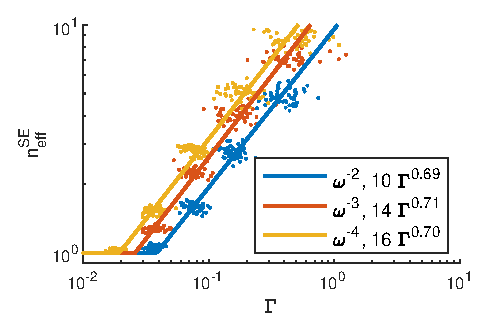
\includegraphics[width=19pc,angle=0]{figures/dofVsGamma}}
  
  \caption{Degrees-of-freedom from the standard error vs $\Gamma$}
  \label{dofVsGamma}
\end{figure}

This idea can be made more rigorous by noting that one would consider change in position, $\Delta x$, statistically significant if exceeds the position errors, $\sigma_x$ by 2-3 factors. Assuming the physical process has a characteristic velocity scale, $u_{\textrm{rms}}$, we use this concept to define $\Gamma$ as
\begin{equation}
\label{gamma_equation}
\Gamma \equiv \frac{\sigma_x}{u_{\textrm{rms}}\Delta t}
\end{equation}
where $\sigma_x$ is the standard deviation of positioning noise and $\Delta t$ is the typical time between observations. this argument suggests that the degrees of freedom is 
\begin{equation}
d_\Gamma = C \Gamma^m.
\end{equation}
Intuitively this means that as long as the particle didn't move too far between observations, nearby observations help to estimate the true position of the particle.

\begin{figure*}[t]
  \centerline{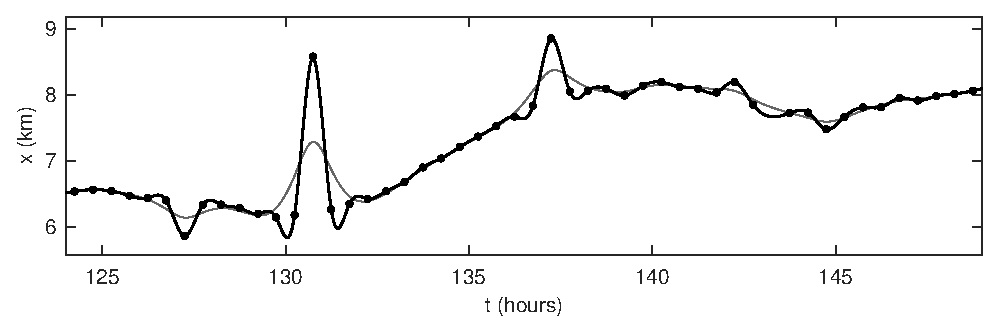
\includegraphics[width=39pc,angle=0]{figures/gaussianfit}}
  
  \caption{An example of model fits to the drifter data assuming Gaussian errors. The thick black line shows a fit with $\sigma=10$ meters, while the gray line shows a fit with $\sigma=50$ meters}
  \label{gaussianfit}
\end{figure*}

The quantity $\Gamma$ can also be interpreted as an interpolation condition. If $\Gamma<1$ then we are in the interpolation regime where the particle moves farther than the measurement noise between observations, and if $\Gamma >1$ we are in the smoothing regime where each observation is providing similar information to nearby observations.

Thus, using the interpolation condition $\Gamma$ to estimate the degrees of freedom, we argue that
\begin{equation}
\label{lambda_initial_guess}
\lambda^{\textrm{initial}}_m = \frac{d_\Gamma-1}{d_\Gamma} \frac{N}{ \left(x^{(m)}_{\textrm{rms}}\right)^2  T}
\end{equation}
should provide a good initial estimate for the optimal smoothing parameter. Section \ref{sec:synthetic_data} shows that indeed this estimate provides an excellent choice of smoothing parameter under a range of conditions.

%%%%%%%%%%%%%%%%%%%%%%
\subsection{Refined degrees-of-freedom} \label{refined_dof}
%%%%%%%%%%%%%%%%%%%%%%

As noted in section \ref{sec:sample_variance}, the degrees of freedom for the sample variance should be the same as the degrees of freedom in the standard error estimate of mean. The standard error estimate for each observation is given by $\mathbf{S_\lambda} \Sigma$ as noted in \ref{sec:numerical_implementation}. The variance of the mean for a Gaussian decreases with increasing degrees of freedom as $\sigma^2/d$, which means that on average then, the number of degrees of freedom in our smoothed path is,
\begin{equation}
d_{\mathbf{S}} = \frac{N}{\Tr \left(\mathbf{S_\lambda} \Sigma \right) }.
\end{equation}
The idea here is then that the tension parameter $\lambda_m$ is adjusted so that,
\begin{equation}
d_\Gamma - d_{\mathbf{S}} = 0
\end{equation}

While we show in section \ref{sec:synthetic_data} that equation \ref{lambda_initial_guess} provides a good initial guess, we find that a more robust approach is to fix the degrees of freedom in the standard error estimate of the mean. In particular the variance of the mean for a Gaussian decreases with increasing degrees of freedom as $\sigma^2/d$. As a vector quantity for each observation this is just $\mathbf{S_\lambda} \Sigma$. On average then, the number of degrees of freedom is,
\begin{equation}
d = \frac{N}{\Tr \left(\mathbf{S_\lambda} \Sigma \right) }.
\end{equation}
Adjusting the tension parameter such that,
\begin{equation}
\label{iterated_tension}
1 + \frac{3 \sigma_x}{u_{\textrm{rms}}\Delta t} = \frac{N}{\Tr \left(\mathbf{S_\lambda} \Sigma \right) }.
\end{equation}
should provide nearly optimal tension.

The difference between the two methods can be summarized as using the degrees of freedom to estimate the variance of the variance, versus using the degrees of freedom to estimate the variance of the mean. Estimating the variance of the mean appears to be more robust.

%%%%%%%%%%%%%%%%%%%%%%
\subsection{Synthetic Data}
\label{sec:synthetic_data}
%%%%%%%%%%%%%%%%%%%%%%

To test these ideas we generate synthetic velocity data from a Gaussian process known as the Matern, and then contaminate the positions with Gaussian noise. The spectrum of the Matern is given by
\begin{equation}
S(\omega) = \frac{A^2}{(\omega^2 + \lambda^2)^\alpha}
\end{equation}
and therefore has finite amplitude low frequency and power-law fall off at high frequencies, two physically realistic properties. For these experiments we choose a value of $\alpha=1$ so that the high frequency spectrum is proportional to $\omega^{-2}$. The Matern is used to generate the \emph{velocity} of the signal and integrated to get the positions and the positions are then contaminated with Gaussian noise. Parameters are chosen such that $u_{\textrm{rms}}=0.20$ m/s and the noise has $\sigma=10$ meters. Figure \ref{synthetic_process_and_spectrum} shows example positions and the velocity spectra of the signal and the noise.

\begin{figure*}[t]
  \centerline{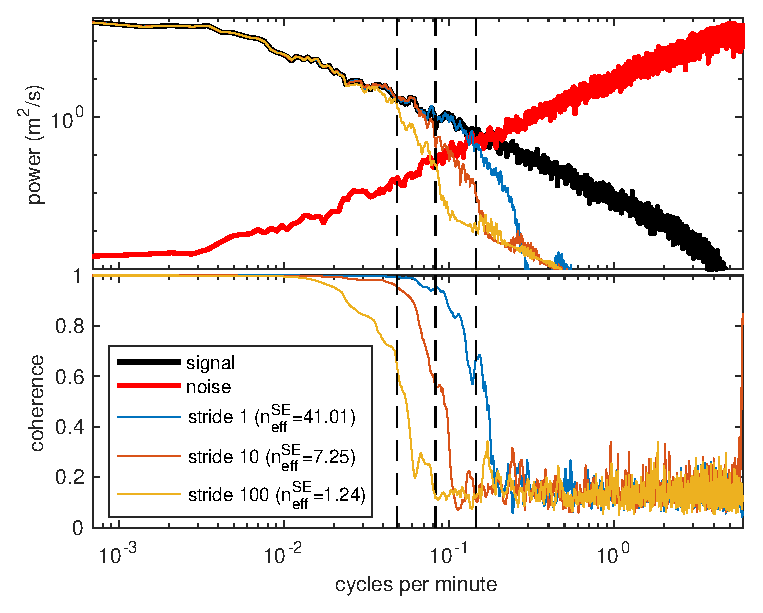
\includegraphics[width=33pc,angle=0]{figures/synthetic_process_and_spectrum_slope2degree3}}
  
  \caption{The upper panel shows the uncontaminated velocity spectrum of the signal (black) and velocity spectrum of the noise (red). The observed signal is the sum of the two. The blue, red, and orange lines show the spectrum of the tension spline best fit to the observations with all, 1/10th and 1/100th the data, respectively. }
  \label{synthetic_process_and_spectrum}
\end{figure*}

For these experiments we choose a spline of degree $S=3$ and apply tension on the second derivative (acceleration). To estimate the tension parameter $\lambda_2$ from equation \ref{lambda} we therefore need an estimate of both $u_{\textrm{rms}}$ and $a_{\textrm{rms}}$. Computing this directly from the observed signal in the time domain is problematic because, given frequent enough sampling, the noise will dominate the estimate. Instead we estimate these values in the frequency domain summing the power in the frequency bins that more than 10 times the expected value of the noise. Because each frequency bin in a periodigram follows a $\chi^2$ distribution for two degrees of freedom, this only adds observed power that is likely to be true signal.

\begin{table}[ht]
\caption{Mean square error and effective degrees-of-freedom for a range of strides (subsampled signal). The first column shows the optimal, best-case scenario found using the uncontaminated signal with 1 dof for each point. The second column shows optimal value using a reduced number of coefficients. This is the lower bound on the error. The iterated estimated found by requiring that equation \ref{iterated_tension} is true. The initial estimate is found using $\lambda_2$ from equation \ref{lambda} directly. }
\label{fit_results}
\centering
\begin{tabular}{r | llll} stride & full dof & reduced dof & blind initial & blind optimal \\ \hline \hline 
-2 slope &&&&  \\ \hline 
2 & 5.18 m$^2$ (20.4) &  -0.1\% (20.6) &  +52.0\% (22.5) &  +1.3\% (20.0) \\ 
8 & 15.0 m$^2$ (7.17) &  +0.2\% (7.05) &  +69.2\% (11.3) &  +0.4\% (7.33) \\ 
32 & 41.5 m$^2$ (2.34) &  -0.0\% (2.50) &  +15.8\% (3.27) &  +0.6\% (2.61) \\ 
128 & 88.9 m$^2$ (1.13) &  -0.0\% (1.16) &  +5.5\% (1.03) &  +1.4\% (1.07) \\ 
-3 slope &&&&  \\ \hline 
2 & 2.73 m$^2$ (30.6) &  -0.1\% (31.6) &  +42.3\% (32.8) &  +2.9\% (30.3) \\ 
8 & 8.48 m$^2$ (11.7) &  -0.0\% (11.8) &  +37.7\% (17.1) &  +0.7\% (12.3) \\ 
32 & 25.4 m$^2$ (3.98) &  +0.1\% (4.07) &  +3.8\% (4.19) &  +0.5\% (3.87) \\ 
128 & 73.7 m$^2$ (1.31) &  +0.0\% (1.30) &  +25.1\% (1.06) &  +1.2\% (1.32) \\ 
-4 slope &&&&  \\ \hline 
2 & 1.78 m$^2$ (53.9) &  -0.2\% (57.3) &  +148.6\% (24.0) &  +5.2\% (45.2) \\ 
8 & 5.61 m$^2$ (16.1) &  -0.2\% (17.4) &  +33.0\% (19.2) &  +0.8\% (15.0) \\ 
32 & 19.1 m$^2$ (5.47) &  +0.1\% (5.43) &  +2.0\% (5.18) &  +1.3\% (4.63) \\ 
128 & 60.6 m$^2$ (1.62) &  -0.0\% (1.63) &  +23.3\% (1.22) &  +1.5\% (1.69) \\ 
\end{tabular} 

\end{table}




To test the accuracy of our method we subsample the observed signal to provide a wide range of effective degrees of freedom, with $\Gamma$ ranging from $0.05$-$30$ corresponding to strides ranging from 512 to 1. The true optimal parameter is determined by minimizing the RMS error between smoothed-interpolated signal and the true signal, as shown in table \ref{fit_results}. Because we are interested interpolation (not just smoothing) the RMS error is computed with all points in the signal, not just those observed in the subsampled signal. This has the result of producing RMS errors that are greater than the standard deviation of the noise (10 meters). The results in table \ref{fit_results} suggest that determining $\lambda$ directly from equation \ref{lambda} and matching degrees-of-freedom with equation \ref{iterated_tension} are both nearly optimal techniques.

\begin{table}[ht]
\caption{Same as above, but with a Student-t distribution }
\label{fit_results}
\centering
\begin{tabular}{r | llll} stride & full dof & reduced dof & blind initial & blind optimal \\ \hline \hline 
m=-2 &&&&  \\ \hline 
2 & 6.45 m$^2$ (17.9) &  -0.1\% (18.9) &  +46.4\% (20.2) &  +1.9\% (24.0) \\ 
8 & 17.8 m$^2$ (7.00) &  +0.2\% (7.41) &  +66.0\% (13.6) &  +0.5\% (7.70) \\ 
32 & 52.1 m$^2$ (2.55) &  +0.0\% (2.71) &  +17.7\% (3.58) &  +1.0\% (2.83) \\ 
128 & 114. m$^2$ (1.13) &  -0.0\% (1.15) &  +1.1\% (1.10) &  +1.1\% (1.13) \\ 
m=-3 &&&&  \\ \hline 
2 & 3.36 m$^2$ (34.9) &  -0.2\% (36.7) &  +92.8\% (34.3) &  +2.6\% (35.2) \\ 
8 & 10.6 m$^2$ (12.1) &  -0.1\% (11.8) &  +30.4\% (14.2) &  +0.8\% (12.3) \\ 
32 & 29.2 m$^2$ (4.06) &  -0.0\% (3.93) &  +7.5\% (4.76) &  +0.6\% (4.13) \\ 
128 & 95.8 m$^2$ (1.39) &  +0.0\% (1.35) &  +14.7\% (1.15) &  +1.9\% (1.30) \\ 
m=-4 &&&&  \\ \hline 
2 & 2.09 m$^2$ (46.5) &  -0.0\% (49.4) &  +124.8\% (54.6) &  +3.6\% (57.1) \\ 
8 & 7.06 m$^2$ (16.3) &  -0.2\% (17.4) &  +37.8\% (23.9) &  +4.6\% (16.5) \\ 
32 & 23.2 m$^2$ (4.88) &  +0.1\% (5.11) &  +3.3\% (5.76) &  +1.0\% (5.40) \\ 
128 & 78.0 m$^2$ (1.68) &  -0.0\% (1.67) &  +12.3\% (1.35) &  +3.2\% (1.45) \\ 
\end{tabular} 

\end{table}

%%%%%%%%%%%%%%%%%%%%%%
\section{GPS data set}
\label{sec:drifter_data_set}
%%%%%%%%%%%%%%%%%%%%%%

The GPS positions used in this manuscript were collected from oceanic surface \emph{drifters}, floating buoys with drogues tethered 15-30 meters below the ocean surface, depending on the particular experiment being conducted. In the past, these drifters have used Argos positioning system which has significantly poorer temporal coverage and position accuracy \cite{elipot2016-jgr}, but recently more surface drifters have employed GPS receivers and transmitted their data back through Argos or Iridium satellites.

The primary dataset considered here will be nine surface drifters that were deployed in the Sargasso Sea in the summer of 2011. These particular drifters were part of the LatMix experiment \cite{shcherbina2015-bams} and recorded data at approximately 30 minute intervals over the course of a week before being retrieved.

The GPS receiver sits on the surface buoy and collects position data, but because of atmospheric conditions or ocean waves, the receivers are sometimes unable to obtain a position, or when they do, it is highly inaccurately. Thus, despite nominal accuracies of a few meters, it is often the case that some positions are off by more than 1000 meters.

In addition to correcting the position errors, it is also important to interpolate the data to a regular grid. Although the sampling period of a GPS receiver can be fixed, because of missing data and time to to acquire signals, the sampling can be quite irregular.  Many analysis techniques require regular sampling (e.g., a Fourier transform) and so it is necessary to interpolate the signal onto a regular grid. The approach taken here is not to simply discard poor data, but also to interpolate the position.



The drifter positions are bivariate time series data given as either projected coordinates $(x_i, y_i)$ or longitude/latitude $(\phi_i, \theta_i$) at times $t_i$. The goal is to create a model of position $(x(t),y(t))$ that is continuous in $t$, and perhaps even continuous for a higher derivative---such as velocity or acceleration---that best matches the data given an assumed set of errors.
%%%%%%%%%%%%%%%%%%%%%%
\subsection{GPS position errors}
%%%%%%%%%%%%%%%%%%%%%%
\label{gps_position_errors}

Figure \ref{gaussianfit} shows a 25 hour window of observed GPS positions for one of the drifters. The bold line in figure \ref{gaussianfit} shows the results of fitting to the observations assuming the errors are Gaussian with $\sigma$ taken to be $10$ meters, while the thin line shows the tension increased by a factor of $10^4$. This increase is equivalent to assuming $1000$ meter standard deviations on the errors---not plausible for ordinary GPS errors, as shown below, and some points must be treated as outliers. 

%%%%%%%%%%%%%%%%%%%%%%
%
\subsection{GPS error distribution}
%
%%%%%%%%%%%%%%%%%%%%%%

We characterize the the GPS errors by considering data from a motionless GPS receiver allowed to run for 12 hours. The specific GPS receiver used for this test was not the same as the one used for the drifters but should produce errors similar enough for this analysis. The errors documented in the FAA GPS accuracy report \cite{faa2016-report} are less comparable because they use superior antennas.

The position recorded by the motionless GPS are assumed to have isotropic errors with mean zero, which means that the positions themselves are the errors. The probability distribution function (PDF) of the combined $x$ and $y$ position errors are shown in figure \ref{motionless_error}.

The error distribution is first fit to a Gaussian PDF,
\begin{equation}
% \label{gaussian_pdf}
p_g(\epsilon|\sigma_g) = \frac{e^{-\frac{1}{2}\frac{\epsilon^2}{\sigma_g^2}} }{\sigma_g \sqrt{ 2 \pi}}.
\end{equation}
The best fit is produced by compute the standard deviation of the sample (Adam, citation?), which is found to be $\sigma_g \approx 10$ meters and shown as the gray line in figure \ref{motionless_error}. However, it is clear the error distribution shows much longer tails than the Gaussian PDF.

The Student t-distribution is a generalization of the Gaussian that produces longer tails and is defined as 
\begin{equation}
\label{student_pdf}
p_t\left(\epsilon |\nu,\sigma_t^2\right) = \frac{\Gamma\left( \frac{\nu + 1}{2} \right)}{\sigma_t \sqrt{\nu \pi} \Gamma\left(\frac{\nu}{2}\right)} \left( 1 + \frac{\epsilon^2}{\sigma_t^2 \nu} \right)^{-\frac{\nu+1}{2}}
\end{equation}
where the $\sigma_t$ parameter scales the distribution width and the $\nu$ parameter sets the number of degrees of freedom. The variance is $\textrm{var}(X)=\sigma_t^2 \frac{\nu}{\nu-2}$ and only exists for $\nu > 2$. The t-distribution is equivalent to the Gaussian distribution when $\nu \rightarrow \infty$. We find the best fit t-distribution to the data by maximizing the Kolmogorov-Smirnoff test. The best fit with parameters $\sigma_t \approx 8.5$ meters and $\nu \approx 4.5$ is shown as the black line in figure \ref{motionless_error}.

\begin{figure}
  \centerline{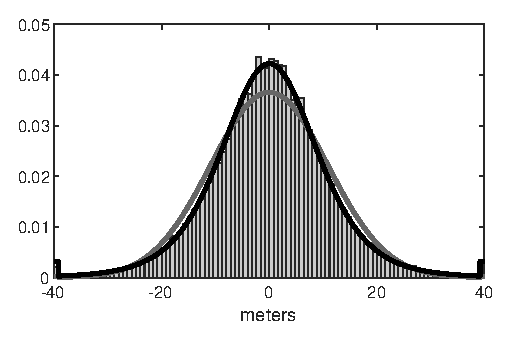
\includegraphics[width=19pc,angle=0]{figures/gps_error_distribution}}
  \centerline{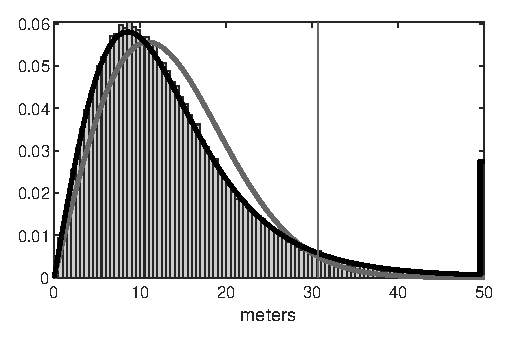
\includegraphics[width=19pc,angle=0]{figures/gps_distance_error_distribution}} 
  \caption{The top panel shows the position error distribution of the motionless GPS. The black line is the best fit t-distribution and the gray line is the best fit Gaussian distribution. The bottom panel shows the distance error distribution with the corresponding expected distributions from the Gaussian and t-distribution. The vertical line in the bottom panel shows the 95\% error of the t-distribution at about 30 meters.}
  \label{motionless_error}
\end{figure}

The \emph{position} error distributions also imply a combined \emph{distance} error distribution by computing $\epsilon_d = \sqrt{\epsilon_x^2 + \epsilon_y^2}$ and is shown in the lower panel of figure \ref{motionless_error}. For two independent Gaussian distributions this results in a Rayleigh distribution,
\begin{equation}
\label{rayleigh_pdf}
p_r(\epsilon_d|\sigma_g) = \frac{\epsilon_d}{\sigma_g^2 } e^{-\frac{1}{2}\frac{\epsilon_d^2}{\sigma_g^2}}.
\end{equation}
The distance distribution for two t-distributions is computed numerically and is shown in the bottom panel of figure \ref{motionless_error}.

\begin{figure}
  \centerline{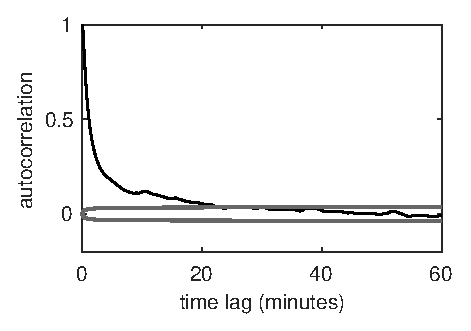
\includegraphics[width=19pc,angle=0]{figures/gps_autocorrelation}}
  \caption{The autocorrelation function of the GPS positioning error with 99\% confidence intervals shown in gray. The correlation at drifter sampling period of 30 minutes is indistinguishable from zero.}
  \label{gps_autocorrelation}
\end{figure}

Figure \ref{gps_autocorrelation} shows the autocorrelation function of the GPS position errors. The smallest sampling interval of the GPS drifters in question is 30 minutes and therefore it is safe to assume the error are uncorrelated for our purposes.

%%%%%%%%%%%%%%%%%%%%%%
%
\subsection{Numerical implementation}
%
%%%%%%%%%%%%%%%%%%%%%%

In practice it is challenging to use the Student t-distribution directly because it does not result in a linear solution for the coefficients like equation \ref{solution}. One method around this issue to use a search algorithm to directly look for the maximum values. Alternatively, one can use the iteratively reweighted least squares (IRLS) method to find the maximum likelihood.

The idea with IRLS to reweight the coefficients of the Gaussian, $\sigma_g$ in equation \ref{gaussian_pdf}, so that the resulting distribution looks like the desired distribution, e.g., equation \ref{student_pdf}. Recalling that $\epsilon_i \equiv x_i - x(t_i,\mathbf{\xi})$, the minimization condition that $\frac{d p_g}{d\xi}=0$, implies that
\begin{equation}
\frac{\epsilon_i}{\sigma_g^2} \frac{\partial x(t_i,\mathbf{x})}{\partial \mathbf{\xi}} = 0
\end{equation}
for the Gaussian distribution, whereas for the t-distribution this implies that,
\begin{equation}
 \frac{\epsilon_i}{\sigma_t^2} \frac{\nu+1}{\nu} \left( 1 + \frac{\epsilon_i^2}{\nu \sigma_t^2} \right)^{-1}  \frac{\partial x(t_i,\mathbf{x})}{\partial \mathbf{\xi}}  = 0.
\end{equation}
This means that you can set
\begin{equation}
\sigma_g^2 =   \sigma_t^2 \frac{\nu}{\nu+1} \left( 1 + \frac{\epsilon_i^2}{\nu \sigma_t^2} \right)
\label{sigma_reweighted}
\end{equation}
to get a matching distribution. Of course, that's only true if $\epsilon_i$ is already known, which initially it is not. So the method becomes iterative---you start with $\epsilon_i$ determined from the Gaussian fit, then determine a new $\epsilon_i$ after reweighting $\sigma_g$. This method iterates until $\sigma_g$ stops changing. We can rewrite equation \ref{sigma_reweighted} as a function of $\epsilon_i$,
\begin{equation}
\label{t-weight}
w_t(\epsilon_i) = \sigma_t^2 \frac{\nu  + \frac{\epsilon_i^2}{\sigma_t^2}}{\nu+1}.
\end{equation}

From equation \ref{t-weight} it is clear that if $\epsilon_i < \sigma_t$ then it will be reweighted to a smaller value, essentially making the observation point more strongly weighted. On the other hand, if $\epsilon_i > \sigma_t$, then its relatively weighting will decrease, and it will be treated more as an outlier.

In a practical sense, the $\Sigma^{-1}$ of equation \ref{smoothing-operator} is replaced with diagonal matrix $W$ populated with the reweighted values for each observation such that,
\begin{equation}
\label{general-smoothing-operator}
\mathbf{S_\lambda} \equiv \mathbf{X} \left[ \mathbf{X}^{\textrm{T}} W \mathbf{X} + \lambda_1 \mathbf{V}^{\textrm{T}} \mathbf{V} \right]^{-1} \mathbf{X}^{\textrm{T}} W.
\end{equation}
This operator is again used to compute the standard error from the variances,  $\mathbf{S_\lambda} \Sigma$, where the variance is assumed to be $\sigma_t^2 \frac{\nu}{\nu-2}$ for each observation.

%%%%%%%%%%%%%%%%%%%%%%
\section{Removing Outliers}
\label{sec:outliers}
%%%%%%%%%%%%%%%%%%%%%%

The goal here is to remove the outliers---points that do not appear to be of the known error distribution for the GPS receiver shown in section \ref{gps_position_errors}. These points are obviously bad as can be seen in figure \ref{gaussianfit} where individual data points jump hundreds of meters and even several kilometers away from its neighbors. Errors of this size are inconsistent with the noise analysis of the preceding section, so the goal here is to first eliminate points associated with this uncharacterized noise. Interestingly, in the nine drifters we are analyzing here, one drifter shows absolutely no obvious outliers, suggesting the issue may be related to how the antenna is configured.

To remove the outliers we use the values of $\nu$ and $\sigma_t$ found in section \ref{gps_position_errors} and set the tension of the spline, \ref{lambda}, by assuming that we have a large number of degrees of freedom. If used for the final product, this will generally result in an overly smoothed fit because the true number of degrees of freedom is much lower. However, this technique will serve to reject outliers because points resulting in an acceleration that is improbably large (according to the Gaussian PDF describing the accelerations) will be treated as having large position errors, a feature that arising from using the Student t-distribution and is not possible if a Gaussian distribution is assumed. Once the fit is performed, the points with errors, $\epsilon_i$, that are far outside the usual bounds can be discarded. 

This technique can be applied independently for the $x$ and $y$ positioning data, but we find that these outlier points are generally correlated, so we base our rejection criteria on the joint distribution, the bottom panel of figure \ref{motionless_error}. We further refine the tension parameter by finding the optimal value of the KS test of the joint distribution, but only within the 99.99\% region. This means that we do not include points that are more than 95 meters away from the model fit in order to avoid fitting to the outliers that do not conform to the model of the motionless GPS. Optimizing the KS test results in a more robust fit because the accelerations estimated using the technique in appendix \ref{variance_estimate} over estimates the acceleration when large outliers are present. Once the tension value is optimized, we then discard the data points outside the 99.99\% of the joint t-distribution.

Once the outliers are removed, the final fits can be performed using \ref{lambda} in conjunction with \ref{iterated_tension}. The thin line in figure \ref{tdistributionfit} shows the final result.

\begin{figure*}[t]
  \centerline{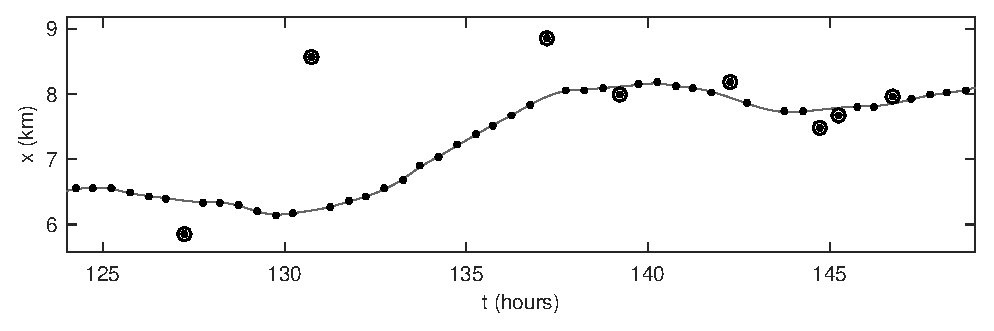
\includegraphics[width=39pc,angle=0]{tdistributionfit}}
  
  \caption{An example of model fits assuming errors following a t-distribution.}
  \label{tdistributionfit}
\end{figure*}


%%%%%%%%%%%%%%%%%%%%%%
\section{Conclusions}
%%%%%%%%%%%%%%%%%%%%%%

- we avoided autocorrelation, although it's very addressable.
- method has strong limitations: stationarity assumptions in particular.
- notice that ultimately we avoid using any interpolation from the interpolating spline, in the sense that we're not using information between the data points. That said, we're still using the 

%%%%%%%%%%%%%%%%%%%%%%
%
\appendices
%
%%%%%%%%%%%%%%%%%%%%%%

%%%%%%%%%%%%%%%%%%%%%%
\section{Numerical implementation}
\label{sec:numerical_implementation}
%%%%%%%%%%%%%%%%%%%%%%

The B-splines are generated using the algorithm described in \cite{deboor1978-book} with knot points determined by equations \ref{even-knots} and \ref{odd-knots}. The matrix $\mathbf{X}$ with components $X\indices{^i_m}$ denotes the $m$-th B-spline at time $t_i$. The first, second and third derivatives of the B-splines are denotes by $V\indices{^i_m}$, $A\indices{^i_m}$, $J\indices{^i_m}$, denoting velocity, acceleration, and jerk, respectively. In this notation the column vector $\xi^m$ represents the coefficients of the splines such that positions at time $t_i$ are given by $\hat{x}^i$ where $\hat{x}^i =  X\indices{^i_m} \xi^m$.

The discretized the penalty function is
\begin{equation}
\begin{split}
\phi = \left[ x^k - X\indices{^k_j} \xi^j \right]^{\textrm{T}} \left(\Sigma^{-1}\right)\indices{^k_i} \left[ x^i - X\indices{^i_l} \xi^l \right] \\
+ \lambda_1 \left[V\indices{^q_j} \xi^j \right]^{\textrm{T}} \left[ V\indices{^q_l} \xi^l \right]
\end{split}
\end{equation}
or
\begin{equation}
\phi = \left[ \mathbf{x} - \mathbf{X} \mathbf{\xi} \right]^{\textrm{T}} \Sigma^{-1} \left[ \mathbf{x} - \mathbf{X} \mathbf{\xi}\right]
+ \lambda_1 \left[\mathbf{V}\mathbf{\xi} - \mu \right]^{\textrm{T}} \left[ \mathbf{V}\mathbf{\xi} - \mu \right]
\end{equation}
where $\Sigma$ denotes the covariance matrix describing the measurement errors.

To find the coefficients that minimize this function, we take the derivative with respect to $\xi^m$, set it equal to zero, and solve for $\xi^m$,
\begin{equation}
\begin{split}
\xi^m = \left[ X\indices{_k_j} \left(\Sigma^{-1}\right)\indices{^k_i}  X\indices{^i_m} + \lambda_1 {A}\indices{^q_j}{A}\indices{^q_m} \right]^{-1} \\
\cdot x_k \left(\Sigma^{-1}\right)\indices{^k_i}   X\indices{^i_j}.
\end{split}
\label{solution}
\end{equation}
or
\begin{equation}
\label{solution2}
\mathbf{\xi} = \left[ \mathbf{X}^{\textrm{T}} \Sigma^{-1} \mathbf{X} + \lambda_1 \mathbf{V}^{\textrm{T}} \mathbf{V} \right]^{-1} \mathbf{X}^{\textrm{T}} \Sigma^{-1} \mathbf{x}
\end{equation}

This means that,
\begin{equation}
\mathbf{\hat{x}} = \mathbf{S_\lambda} \mathbf{x}
\end{equation}
where we've defined the smoothing matrix
\begin{equation}
\label{smoothing-operator}
\mathbf{S_\lambda} \equiv \mathbf{X} \left[ \mathbf{X}^{\textrm{T}} \Sigma^{-1} \mathbf{X} + \lambda_1 \mathbf{V}^{\textrm{T}} \mathbf{V} \right]^{-1} \mathbf{X}^{\textrm{T}} \Sigma^{-1}.
\end{equation}
which takes observations $\mathbf{x}$ to their smoothed values $\mathbf{\hat{x}}$.

The first matrix on the right hand side of equation \ref{solution} is $N\times N$ and fully invertible because the knots point were chosen such that each spline has at least one data point in its nonzero region. This is a nice feature because it means the solution will be well-behaved even if there is no tension.

%%%%%%%%%%%%%%%%%%%%%%
\section{Spline with mean tension}
%%%%%%%%%%%%%%%%%%%%%%
\label{mean_tension}

The tension spline condition given in \ref{gaussian-max-likelihood-penalty} can be augmented to include a nonzero mean tension, $\mu_u$,
\begin{equation}
\phi =  \frac{d}{d-1} \frac{1}{N} \sum^N _{i=1}\left( \frac{x_i - x(t_i)}{\sigma_i} \right)^2 + \frac{1}{Q} \sum^{Q}_{q=1}  \left(  \frac{u(t_q)-\mu_u}{\sigma_u} \right)^2.
\end{equation}
When discretized, this penalty function becomes
\begin{equation}
\phi = \left[ \mathbf{x} - \mathbf{X} \mathbf{\xi} \right]^{\textrm{T}} \Sigma^{-1} \left[ \mathbf{x} - \mathbf{X} \mathbf{\xi}\right]
+ \lambda_1 \left[\mathbf{V}\mathbf{\xi} - \mu \right]^{\textrm{T}} \left[ \mathbf{V}\mathbf{\xi} - \mu \right]
\end{equation}
which has solution
\begin{equation}
\mathbf{\xi} = \left[ \mathbf{X}^{\textrm{T}} \Sigma^{-1} \mathbf{X} + \lambda_1 \mathbf{V}^{\textrm{T}} \mathbf{V} \right]^{-1}   \left[ \mathbf{X}^{\textrm{T}} \Sigma^{-1} \mathbf{x} +  \mu \lambda_1 \mathbf{V}^{\textrm{T}} \mathbf{\iota} \right]
\end{equation}
where $\mathbf{\iota}$ is a vector of $1$s. The operation $\mathbf{V}^{\textrm{T}} \mathbf{\iota}$ essentially integrates the $m$-splines and results in a column vector with the integrated values.


%%%%%%%%%%%%%%%%%%%%%%
\section{Estimating the variance of the signal}
%%%%%%%%%%%%%%%%%%%%%%
\label{variance_estimate}

The method in this paper depends on good estimates of the root-mean-square velocity, $u_{\textrm{rms}}$, of the signal in order to determine the effective degrees of freedom, as well as variance of the tensioned derivative, $a_{\textrm{std}}^2$, for example. The approach taken here is to compute power spectrum of the signal at the derivative of interest, and sum the variance that is statistically significantly greater than the expected variance of the noise.

Given a process observed with values $x_n$ at times $t_n = n \Delta$ where $n=1..N$, we estimate the mean of its $m$-th derivative by performing a least squares fit to the polynomial $\bar{x}_n \equiv p_m t_n^m + p_{m-1} t_n^{m-1} + .. + p_0$. The \emph{detrended} time series is then defined as $\tilde{x}_n \equiv x_n - \bar{x}_n$. The power spectrum of this time series is given by
\begin{equation}
S_{\textrm{signal}}(f_k) = \frac{\Delta}{N} \left\lvert \sum_{n=0}^{N-1} x_n e^{-2\pi i f_k t_n} \right\rvert^2
\end{equation}
where the frequencies $f_k$ are given by $f_k = \frac{k}{N\Delta}$. When unwrapped to include negative values, $f_k = \frac{1}{N \Delta} \left[ -\left\lfloor \frac{N}{2} \right\rfloor,...,\left\lceil \frac{N}{2} \right\rceil -1 \right]$. By Plancherel's theorem,
\begin{equation}
\label{plancherel}
\sum_{k=0}^{N-1} S(f_k) \cdot \frac{1}{N \Delta} = \frac{1}{N \Delta} \sum_{i=0}^{N-1} x_i^2 \Delta.
\end{equation}
The power spectrum of the $m$-th derivative of the process is computed as,
\begin{equation}
S_{\textrm{signal}}^{(m)}(f_k) = (2 \pi f_k)^{2m} \cdot S(f_k).
\end{equation}
Note that it is important to detrend the signal prior to computing the derivative because, by assumption, the signal is periodic and has no secular trend.

The noise, $\epsilon_i$, has total variance $\sigma^2 = \frac{1}{N} \sum_{i=1}^{N} \epsilon_i^2$. Because the noise is assumed to be uncorrelated, the variance distributes evenly across all frequency. The spectrum of the noise is therefore,
\begin{equation}
S_{\textrm{noise}}(f_k) = \sigma^2 \Delta
\end{equation}
which immediately can be seen to satisfy Plancherel's theorem \ref{plancherel}. The $m$-th derivative of the noise has the power spectrum
\begin{equation}
S_{\textrm{noise}}^{(m)}(f_k) = \sigma^2 \Delta (2 \pi f_k)^{2m}.
\end{equation}

The technique used here sums the variance of the signal for a given frequency if it exceeds the expected variance of the noise at the frequency by some threshold. The estimate of power at each frequency follows a $\chi^2$ distribution with 2 degrees-of-freedom, so we choose the threshold based on the 95-th percentile of the expected distribution. And thus,
\begin{equation}
x^{(m)}_{\textrm{std}} = \sum_{k=1}^{N} S^{(m)}_{\textrm{signal}}(f_k) \cdot \left( S^{(m)}_{\textrm{signal}}(f_k) > q S_{\textrm{noise}}^{(m)}(f_k) \right) \cdot \frac{1}{N \Delta}
\end{equation}
where $q\approx 20$ for the 95 percent confidence.

\section*{Acknowledgment}
Thanks to my funding agencies and to collaborators. 

\bibliographystyle{IEEEtranBST/IEEEtran}
\bibliography{references}

\end{document}